\appendix

\section{Appendiks - Forklaring på segfault}\label{app:segfault}

Når dere kompilerer et program, vil dere til slutt ende opp med noe som ligner på figur \ref{fig:4-minne-struktur}. Programmet er delt opp i områder med forskjellige rettigheter. Feltet \verb|.text| er minne-området som inneholder maskinkoden som faktisk kjører, samt statisk lenkede biblioteker. Dette området krever lese- og kjørerettigheter, men vi har virkelig ikke lyst til å gi området skriverettigheter - fordi programmet da potensielt kunne ha skrevet om seg selv.

\begin{figure}[ht]
    \centering
    

\tikzset{every picture/.style={line width=0.75pt}} %set default line width to 0.75pt        

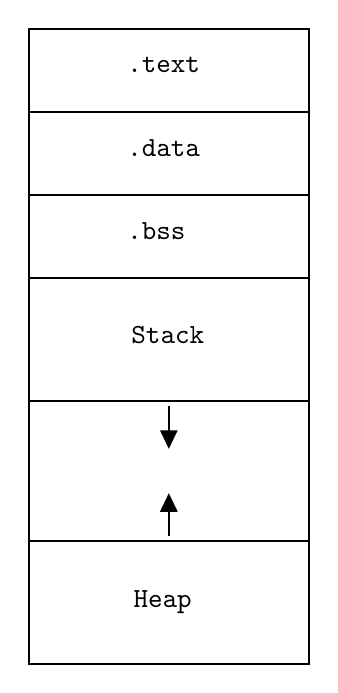
\begin{tikzpicture}[x=0.75pt,y=0.75pt,yscale=-1,xscale=1]
%uncomment if require: \path (0,339); %set diagram left start at 0, and has height of 339

%Shape: Rectangle [id:dp13101589938105973] 
\draw   (243,10) -- (378,10) -- (378,50) -- (243,50) -- cycle ;
%Shape: Rectangle [id:dp06368153206435134] 
\draw   (243,50) -- (378,50) -- (378,90) -- (243,90) -- cycle ;
%Shape: Rectangle [id:dp8533115917784224] 
\draw   (243,90) -- (378,90) -- (378,130) -- (243,130) -- cycle ;
%Shape: Rectangle [id:dp04455868614862735] 
\draw   (243,130) -- (378,130) -- (378,189.2) -- (243,189.2) -- cycle ;
%Shape: Rectangle [id:dp9354652197962545] 
\draw   (243,257) -- (378,257) -- (378,316.2) -- (243,316.2) -- cycle ;
%Straight Lines [id:da9885326185507459] 
\draw    (243,189.2) -- (243,257) ;
%Straight Lines [id:da5770026001630877] 
\draw    (378,189.2) -- (378,257) ;
%Straight Lines [id:da33638011482323815] 
\draw    (310.5,191.6) -- (310.5,209.4) ;
\draw [shift={(310.5,212.4)}, rotate = 270] [fill={rgb, 255:red, 0; green, 0; blue, 0 }  ][line width=0.08]  [draw opacity=0] (8.93,-4.29) -- (0,0) -- (8.93,4.29) -- cycle    ;
%Straight Lines [id:da3195032750258344] 
\draw    (310.5,236.8) -- (310.5,254.6) ;
\draw [shift={(310.5,233.8)}, rotate = 90] [fill={rgb, 255:red, 0; green, 0; blue, 0 }  ][line width=0.08]  [draw opacity=0] (8.93,-4.29) -- (0,0) -- (8.93,4.29) -- cycle    ;

% Text Node
\draw (289,22) node [anchor=north west][inner sep=0.75pt]   [align=left] {\texttt{.text}};
% Text Node
\draw (289,62) node [anchor=north west][inner sep=0.75pt]   [align=left] {\texttt{.data}};
% Text Node
\draw (289,102) node [anchor=north west][inner sep=0.75pt]   [align=left] {\texttt{.bss}};
% Text Node
\draw (291,152) node [anchor=north west][inner sep=0.75pt]   [align=left] {\texttt{Stack}};
% Text Node
\draw (292,279) node [anchor=north west][inner sep=0.75pt]   [align=left] {\texttt{Heap}};


\end{tikzpicture}
    \caption{Vanlig minne-struktur for et program.}
    \label{fig:4-minne-struktur}
\end{figure}

Feltet \verb|.data| og \verb|.bss| inneholder henholdsvis \textit{compile time} initialisert-allokert og uinitialisert minne. Disse feltene er for globale variabler.

\verb|Heap|-feltet er området minne-kall til \verb|malloc| og \verb|free| vil virke på. \verb|Heap|-en er for dynamisk allokert minne, og vil vokse oppover dersom en gjennom kall til \verb|malloc| bruker opp allokert \verb|heap|-størrelse.

Ovenfor \verb|heap|-en ligger området for \verb|stack|-en. Denne vil bestå av såkalte \verb|stack|-frames med lokale variabler. Om du gjør uendelig rekursjon i et språk som ikke støtter \textit{tail recursion}, så vil \verb|stack|-en vokse nedover til den til slutt kolliderer med \verb|heap|-en. Dette er det som kalles en \textit{stack overflow}.

Nøyaktig hvor dynamisk lenkede biblioteker ligger, og hvor kopier av eksterne variabler finnes, er implementasjonsspesifikt - men de generelle trekkene i figur \ref{fig:4-minne-struktur} stemmer som regel.

Når dere kjører et program vil dere som regel ikke jobbe direkte med informasjon som er lagret på harddisk eller annet sekundærminne. Grunnen til dette er at både skriving til og lesing fra datamaskinens primærminne som ofte består av RAM (\textbf{R}andom \textbf{A}ccess \textbf{M}emory) er betydelig raskere enn til og fra harddisken. Under kjøring av et program laster derfor datamaskinen deler av informasjon fra sekundærminne til primærminne, altså typisk fra harddisk til RAM. Disse delene kalles \textit{memory pages}, og størrelsen på disse er avhengig av arkitektur. Operativsystemet vil gi hver \textit{memory page} diverse flagg for å holde styr på hva man kan gjøre med minnet.

Uheldigvis er det ganske vanlig at man har et array som ikke tar en hel \textit{page}. Dermed kan man gjøre ulovlige minne-operasjoner så lenge man er `heldig' og treffer en \textit{page} som man har aksess-rettigheter til. En \textit{out-of-bounds} på ett element vil derfor ikke alltid gi en segfault, som det burde.

\section{Appendiks - Debugging av mikrokontrollere}\label{app:debugg-micro}
Det er mulig å bruke GDB for å debugge mikrokontrollere, så lenge man har en måte å kommunisere debuggingssignaler til hardwaret. I tillegg må hardwaret også støtte debugging, men dette er stort sett garantert i nye mikrokontrollere. Det er mange måter å gå frem - men her er en rask innføring som viser hvordan man kan debugge micro:bit-en som er brukt i faget med SWD (\textbf{s}ingle \textbf{w}ire \textbf{d}ebugging). Framgangsmåten for å debugge mikrokontrollere er forskjellig fra plattform til plattform ettersom de har ulike debuggingsgrensesnitt, men som oftest er Google veldig behjelpelig om  man søker: \verb|"How to set up GDB server on ..."|.

\subsection{Server}

Det første som kreves i det generelle tilfellet er et serverprogram som kjører på målhardwaret som blir debugget. Dette vil tillate en GDB-klient å koble seg til over en seriell linje, eller over en TCP/IP-forbindelse. Fordi micro:bit-en allerede støtter SWD, trenger man ikke å kompilere serveren selv. En kan da bruke andre verktøy som er i stand til å bruke SWD, og så koble GDB-klienten til dette verktøyet (se figur \ref{fig:4-SWD-connection})

\begin{figure}[ht]
    \centering
    

\tikzset{every picture/.style={line width=0.75pt}} %set default line width to 0.75pt        

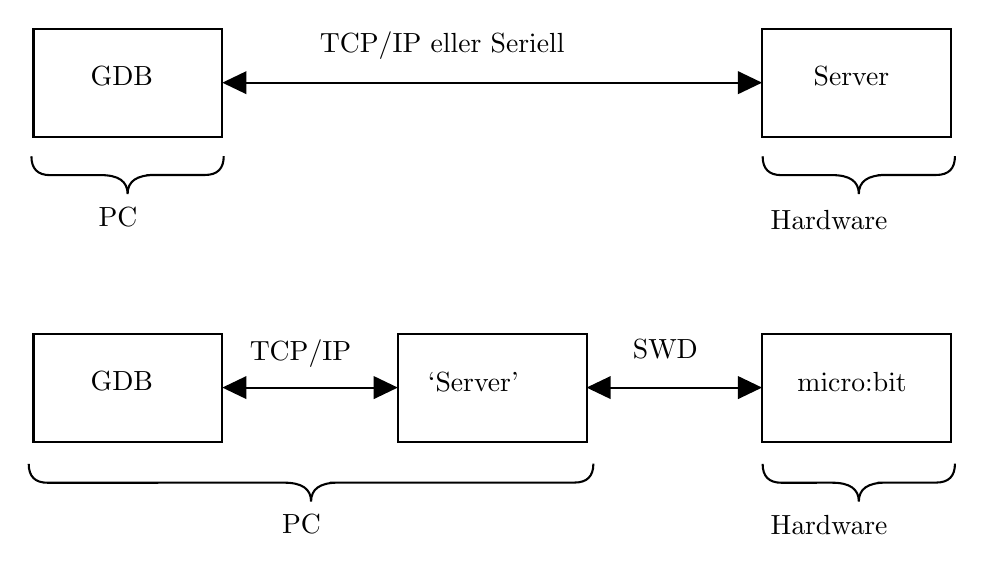
\begin{tikzpicture}[x=0.75pt,y=0.75pt,yscale=-1.3,xscale=1.3]
%uncomment if require: \path (0,300); %set diagram left start at 0, and has height of 300

%Shape: Rectangle [id:dp2040495981987429] 
\draw   (276,162) -- (346,162) -- (346,202) -- (276,202) -- cycle ;
%Shape: Rectangle [id:dp8791019060072369] 
\draw   (141,162) -- (211,162) -- (211,202) -- (141,202) -- cycle ;
%Shape: Rectangle [id:dp34562906859358766] 
\draw   (411,162) -- (481,162) -- (481,202) -- (411,202) -- cycle ;
%Shape: Rectangle [id:dp10020003065736183] 
\draw   (141,49) -- (211,49) -- (211,89) -- (141,89) -- cycle ;
%Shape: Rectangle [id:dp4454199949106217] 
\draw   (411,49) -- (481,49) -- (481,89) -- (411,89) -- cycle ;
%Straight Lines [id:da46711444160880555] 
\draw    (214,69) -- (408,69) ;
\draw [shift={(411,69)}, rotate = 180] [fill={rgb, 255:red, 0; green, 0; blue, 0 }  ][line width=0.08]  [draw opacity=0] (8.93,-4.29) -- (0,0) -- (8.93,4.29) -- cycle    ;
\draw [shift={(211,69)}, rotate = 0] [fill={rgb, 255:red, 0; green, 0; blue, 0 }  ][line width=0.08]  [draw opacity=0] (8.93,-4.29) -- (0,0) -- (8.93,4.29) -- cycle    ;
%Shape: Brace [id:dp12694272910051874] 
\draw   (140.23,96.27) .. controls (140.23,100.94) and (142.56,103.27) .. (147.23,103.27) -- (165.87,103.25) .. controls (172.54,103.24) and (175.87,105.57) .. (175.88,110.24) .. controls (175.87,105.57) and (179.2,103.23) .. (185.87,103.22)(182.87,103.23) -- (204.51,103.21) .. controls (209.18,103.2) and (211.51,100.87) .. (211.5,96.2) ;
%Shape: Brace [id:dp849533451177146] 
\draw   (411.23,96.27) .. controls (411.23,100.94) and (413.56,103.27) .. (418.23,103.27) -- (436.87,103.25) .. controls (443.54,103.24) and (446.87,105.57) .. (446.88,110.24) .. controls (446.87,105.57) and (450.2,103.23) .. (456.87,103.22)(453.87,103.23) -- (475.51,103.21) .. controls (480.18,103.2) and (482.51,100.87) .. (482.5,96.2) ;
%Shape: Brace [id:dp048064701846972424] 
\draw   (139.23,210.27) .. controls (139.23,214.94) and (141.56,217.27) .. (146.23,217.27) -- (233.87,217.24) .. controls (240.54,217.24) and (243.87,219.57) .. (243.87,224.24) .. controls (243.87,219.57) and (247.2,217.24) .. (253.87,217.23)(250.87,217.23) -- (341.5,217.2) .. controls (346.17,217.2) and (348.5,214.87) .. (348.5,210.2) ;
%Shape: Brace [id:dp19293139300351636] 
\draw   (411.23,210.27) .. controls (411.23,214.94) and (413.56,217.27) .. (418.23,217.27) -- (436.87,217.25) .. controls (443.54,217.24) and (446.87,219.57) .. (446.88,224.24) .. controls (446.87,219.57) and (450.2,217.23) .. (456.87,217.22)(453.87,217.23) -- (475.51,217.21) .. controls (480.18,217.2) and (482.51,214.87) .. (482.5,210.2) ;
%Straight Lines [id:da7052759156801001] 
\draw    (214,182) -- (273,182) ;
\draw [shift={(276,182)}, rotate = 180] [fill={rgb, 255:red, 0; green, 0; blue, 0 }  ][line width=0.08]  [draw opacity=0] (8.93,-4.29) -- (0,0) -- (8.93,4.29) -- cycle    ;
\draw [shift={(211,182)}, rotate = 0] [fill={rgb, 255:red, 0; green, 0; blue, 0 }  ][line width=0.08]  [draw opacity=0] (8.93,-4.29) -- (0,0) -- (8.93,4.29) -- cycle    ;
%Straight Lines [id:da7465676171907607] 
\draw    (349,182) -- (408,182) ;
\draw [shift={(411,182)}, rotate = 180] [fill={rgb, 255:red, 0; green, 0; blue, 0 }  ][line width=0.08]  [draw opacity=0] (8.93,-4.29) -- (0,0) -- (8.93,4.29) -- cycle    ;
\draw [shift={(346,182)}, rotate = 0] [fill={rgb, 255:red, 0; green, 0; blue, 0 }  ][line width=0.08]  [draw opacity=0] (8.93,-4.29) -- (0,0) -- (8.93,4.29) -- cycle    ;

% Text Node
\draw (286,175) node [anchor=north west][inner sep=0.75pt]   [align=left] {`Server'};
% Text Node
\draw (161,175) node [anchor=north west][inner sep=0.75pt]   [align=left] {GDB};
% Text Node
\draw (423,175) node [anchor=north west][inner sep=0.75pt]   [align=left] {micro:bit};
% Text Node
\draw (161,62) node [anchor=north west][inner sep=0.75pt]   [align=left] {GDB};
% Text Node
\draw (429,62) node [anchor=north west][inner sep=0.75pt]   [align=left] {Server};
% Text Node
\draw (246,49) node [anchor=north west][inner sep=0.75pt]   [align=left] {TCP/IP eller Seriell};
% Text Node
\draw (164,114) node [anchor=north west][inner sep=0.75pt]   [align=left] {PC};
% Text Node
\draw (232,228) node [anchor=north west][inner sep=0.75pt]   [align=left] {PC};
% Text Node
\draw (413,115) node [anchor=north west][inner sep=0.75pt]   [align=left] {Hardware};
% Text Node
\draw (413,228) node [anchor=north west][inner sep=0.75pt]   [align=left] {Hardware};
% Text Node
\draw (362,163) node [anchor=north west][inner sep=0.75pt]   [align=left] {SWD};
% Text Node
\draw (220,163) node [anchor=north west][inner sep=0.75pt]   [align=left] {TCP/IP};


\end{tikzpicture}
    \caption{Skjematisk illustrasjon av GDB sitt grensesnitt mot micro:bit-en.}
    \label{fig:4-SWD-connection}
\end{figure}


Her tar `Server'-enheten seg av kommunikasjon med både GDB, og hardware, ved å abstrahere bort hvilken type forbindelse man har mellom datamaskinen og plattformen som blir debugget. 

I prinsippet kan `Server' være hva som helst, så lenge det er et program som støtter kommandoer fra GDB, og er i stand til å kommunisere med målhardwaret. Programvaren OpenOCD (\textbf{Open} \textbf{O}n-\textbf{C}hip-\textbf{D}ebugger) er et godt valg her, og er den programvaren vi vil bruke i dette eksemplet.

\subsection{Overføre koden vi ønsker å debugge}
I eksempelmappen \verb|example_microbit| ligger det en simpel kode som dere kan kompiler og flashe ved å kalle \verb|make ; make flash|. Koden vil toogle LED-matrisen på hver rad så fort micro:bit-en kan.

\subsection{OpenOCD}

OpenOCD lar brukeren spesifisere hvordan vi skal kommunisere med hardware over en form for kobling som støtter debugging - eksempelvis JTAG, CMSIS-DAP, USB-Blaster, eller i vårt tilfelle; SWD.

Før vi kan bruke OpenOCD, må vi installere programmet. Dette kan gjøres ved å kalle \verb|sudo apt install openocd| på datamaskinene på Sanntidssalen. 

OpenOCD kan startes på to måter. Man kan enten spesifisere alle parametrene som er nødvendige for å definere kommunikasjonsprotokollen via kommandolinjen, eller man kan opprette en konfigurasjonsfil kalt \verb|openocd.cfg| i mappen man har prosjektet i. For gjenbrukbarhetens skyld er det bedre å benytte seg av konfigurasjonsfilen.

I vårt tilfelle skal \verb|openocd.cfg| se slik ut:

\begin{lstlisting}[mathescape=true]
interface jlink
transport select swd

source [find target/nrf51.cfg]

gdb_memory_map enable
\end{lstlisting}


Deretter starter vi koblingen mellom datamaskin og micro:biten ved å kalle \verb|sudo openocd| fra samme mappe som konfigurasjonsfilen ligger. Dette vil gi en output som ligner denne:

\begin{lstlisting}[mathescape=true]
Open On-Chip Debugger 0.10.0
Licensed under GNU GPL v2
For bug reports, read
        http://openocd.org/doc/doxygen/bugs.html
cortex_m reset_config sysresetreq
adapter speed: 1000 kHz
Info : No device selected, using first device.
Info : J-Link OB-BBC-microbit compiled Mar 24 2017 09:33:30
Info : Hardware version: 1.00
Info : VTarget = 3.300 V
Info : clock speed 1000 kHz
Info : SWD DPIDR 0x0bb11477
Info : nrf51.cpu: hardware has 4 breakpoints, 2 watchpoints
\end{lstlisting}


Dette betyr at OpenOCD er nå klar for å motta forespørsler over TCP/IP, som GDB kan koble seg til via. Om dere ikke spesifiserer noe annet, vil OpenOCD lytte på port 3333. \textcolor{RWTHrot100}{\textbf{Dere kan ikke bruke \texttt{nrfjprog} og \texttt{openocd} samtidig. Dere må altså lukke \texttt{openocd} før dere kaller \texttt{make flash}. Dette er igjen grunnet begrensninger i JLink-firmwaren på micro:bit-en!}}

\subsection{Debugging av micro:bit med GDB}

Dersom alt har blitt satt opp riktig, burde dere kunne starte GDB fra samme mappe, ved å kalle \verb|arm-none-eabi-gdb build/main.elf -iex "target remote| \verb| localhost:3333" -tui|. Vi bruker her \verb|arm-none-eabi|-prefikset for å spesifisere at dette er GDB bygget på ARM-baserte arkitekter, i motsetning til x86-64, som vi ellers bruker.



Dersom man nå fra GDB kaller \verb|monitor reset halt|, etterfulgt av \verb|break main|, og deretter \verb|continue|, vil programmet på micro:bit-en kjøre gjennom oppstartskoden og stoppe ved første instruksjon i \verb|main|. I dette tilfellet er første instruksjon i \verb|main| definert som \verb|for|-løkken som konfigurer matrisen på micro:bit-en.

Man kan nå kalle \verb|until| et par ganger, til dere stopper på første linje i \verb|while|-løkka. Dette kan ta litt tid, eventuelt kan det \textit{lagge} litt. Når man har kommet ned til \verb|GPIO->OUTSET...|, kan man bruke \verb|next| til å stoppe gjennom hver operasjon og se at matrisen på micro:bit-en skrur seg på- og av en rad av gangen.


Stort sett er alle operasjonene som er tilgjengelig i vanlig GDB nå tilgjengelige for bruk på micro:bit-en. I tillegg til disse har man også en del hardwarespesifikke kommandoer; disse starter med \verb|monitor [...]|, eksempelvis kommandoen \verb|monitor reset halt|, som vil starte målet på nytt, og med en gang fryse programflyten.